\documentclass{lxaiproposal}

\usepackage[english]{babel}

\PassOptionsToPackage{hyphens}{url}\usepackage{hyperref}
\usepackage{times}
\usepackage{array}
\usepackage{color}
\usepackage{epsfig}
\usepackage{pifont}
\usepackage{pifont}
\usepackage{caption}
\usepackage{float}
\usepackage{amsmath}
\usepackage{amssymb}
\usepackage{caption}
\usepackage{amssymb}
\usepackage{pdfpages}
\usepackage{makecell}
\usepackage{booktabs}
\usepackage{latexsym}
\usepackage{booktabs}
\usepackage{colortbl}
\usepackage{multirow}
\usepackage{tabularx}
\usepackage{subcaption}

\usepackage[T1]{fontenc}
\usepackage[latin1]{inputenc}

\title{Virtual Node Graph Neural Networks for Hypothetical Metal Organic Framework Inference Tasks\\ \large Summer 2023 PURA Salary Award Proposal}

\author{\coord{Sidharth Baskaran}{}{1}}

\address{\affil{1}{
College of Computing, Georgia Institute of Technology}}

\email{sidharth.baskaran@gatech.edu}

\begin{document}
\maketitle

\section*{Project Overview}

In materials science, molecular property prediction has a range of applications, including
energy catalyst optimization and drug materials discovery. Graph neural networks (GNNs) have proven to be effective for such inference tasks; structurally representing molecules as graphs and scaling to $O(n)$ runtime complexity as opposed to $O(n^3)$ for one of the most popular conventional methods, density-functional theory (DFT). Metal-organic frameworks (MOFs) are porous materials consisting of metal clusters linked by organic components, and pose a challenge for GNNs due to difficulty in expressing pores in graph structures. We propose a model-agnostic method incorporating virtual nodes into molecular graphs for improved expressiveness and performance on MOF prediction tasks that has shown promising results to date.
This project is undertaken under mentorship of Dr. Victor Fung (\textit{Georgia Tech CSE}) and in collaboration with Dr. Guojing Cong (\textit{Oak Ridge National Laboratory}).

\subsection*{Message-Passing Graph Neural Networks}

Graph neural networks (GNNs) have become increasingly popular in the materials science space, and can be used on a variety of tasks, including property inference, synthesis prediction, and structure generation\cite{Reiser2022}. In principle, GNNs are able to perform convolutions over arbitrary inputs with standardized feature dimensions, and offer the advantage of working with atomic structures that easily translate to graphs. Message-passing (MP) GNNs propagate information between adjacent nodes across bonds, a concept used in modern graph convolutional operators such as in CGCNN\cite{Xie_2018}. Each atom in a structure is a node in the graph, and is assigned a vector of node attributes encoding chemical and neighboring properties. Bonds are represented by edges and are assigned vectorial attributes encoding spatial information (\ref{fig:vec-reps}). Molecular property inference involves scalar-valued predictions given graph inputs. A common pipeline involves a series of convolutional layers followed by a set of fully-connected classification layers to provide a global readout value (\ref{fig:e2e}).

\begin{figure*}[h]
    \centering
    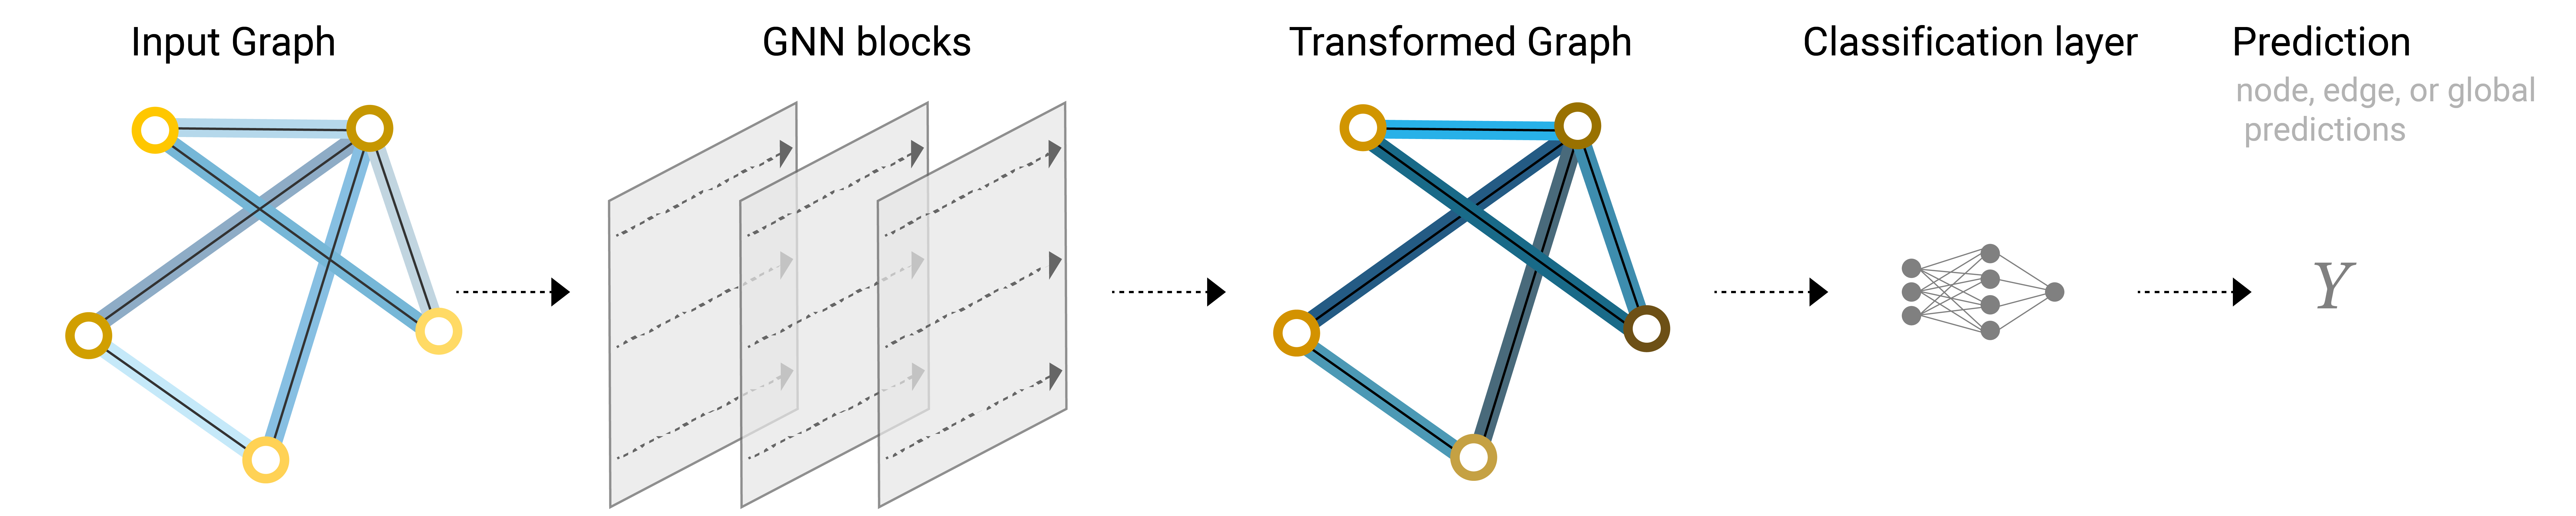
\includegraphics[scale=0.4]{gnn-e2e.png}
    \caption{End-to-end GNN property inference task\cite{sanchez-lengeling2021a}}
    \label{fig:e2e}
\end{figure*}

\begin{figure*}
    \centering
    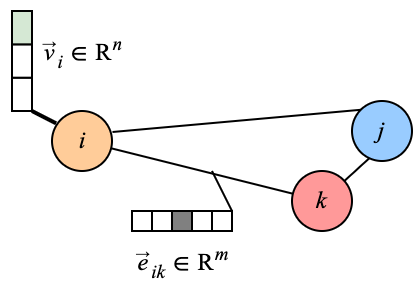
\includegraphics[scale=0.4]{graph-rep.drawio.png}
    \caption{Node and edge vector attributes}
    \label{fig:vec-reps}
\end{figure*}

\subsection*{hMOF Dataset}

Metal-organic frameworks (MOFs) are composed of modular building blocks that form crystal structures, and are of interest due to their porous nature among other properties. The space of  MOFs is large due to their modular structure, which allows for millions of possible structures. The hypothetical metal-organic framework (hMOF) generation procedure generates every possible structure under constraints to produce 137,953 hMOFs, using building blocks of naturally occurring MOFs. The global properties for each structure are surface area, pore volume, pore-size distribution, powder X-ray diffraction pattern, and methane-adsorption capability\cite{wilmer2012large}.

\subsection*{Virtual Nodes for Graph Structures}

Crystal structures are an infinite system, and GNNs use the smallest repeating unit (unit cell) as an approximation for the system. Virtual nodes can be situated along the 3D boundary conditions describing the unit cell to form a controllable mesh. Each virtual node is described by a node attribute vector and is connected via edges to real and virtual nodes.

\section*{Project objective and goals}

\section*{Research Plan and Methods}

\subsection{Preliminary Results}

\subsection{Outperforming Baseline Results}

\subsection{Incorporating Heterogeneous Graphs}

\section*{Related Work}

Machine learning-based approaches to predict methane-adsorption exist, but do not utilize GNNs, rather creating structural fingerprint vectors encoding spatial and chemical information. Deep neural networks are then used to map these fingerprints to predicted methane-adsorption. \cite{gurnani2021interpretable}. 
Virtual nodes have been used in GNNs for materials property inference, but for different use cases including full phonon\cite{https://doi.org/10.48550/arxiv.2010.09435} and electron density prediction\cite{jorgensen2022equivariant}.

\section*{Projected Outcome and Implications}

Anand Radhakrishnan and I will arrive on Sunday, November 13, 2022, and return to Atlanta on Thursday, November 17, 2022. We plan on attending many events held at the conference and thus chose to leave Atlanta on Sunday rather than on Monday morning. This has the added benefit of protecting us from unforeseen events such as flight cancellations.

\section*{Acknowledgments}

This work used OLCF Summit under Director's Discretionary allocation CFD154 and
XSEDE resources under allocation TG-PHY210084.
We also acknowledge hardware awards from the NVIDIA Academic Hardware Grants
program.

\bibliographystyle{ieee_fullname}
\bibliography{references}

\end{document}